\documentclass[tikz,border=2pt]{standalone}
\usetikzlibrary{arrows.meta,positioning,calc,shapes.geometric}

\begin{document}
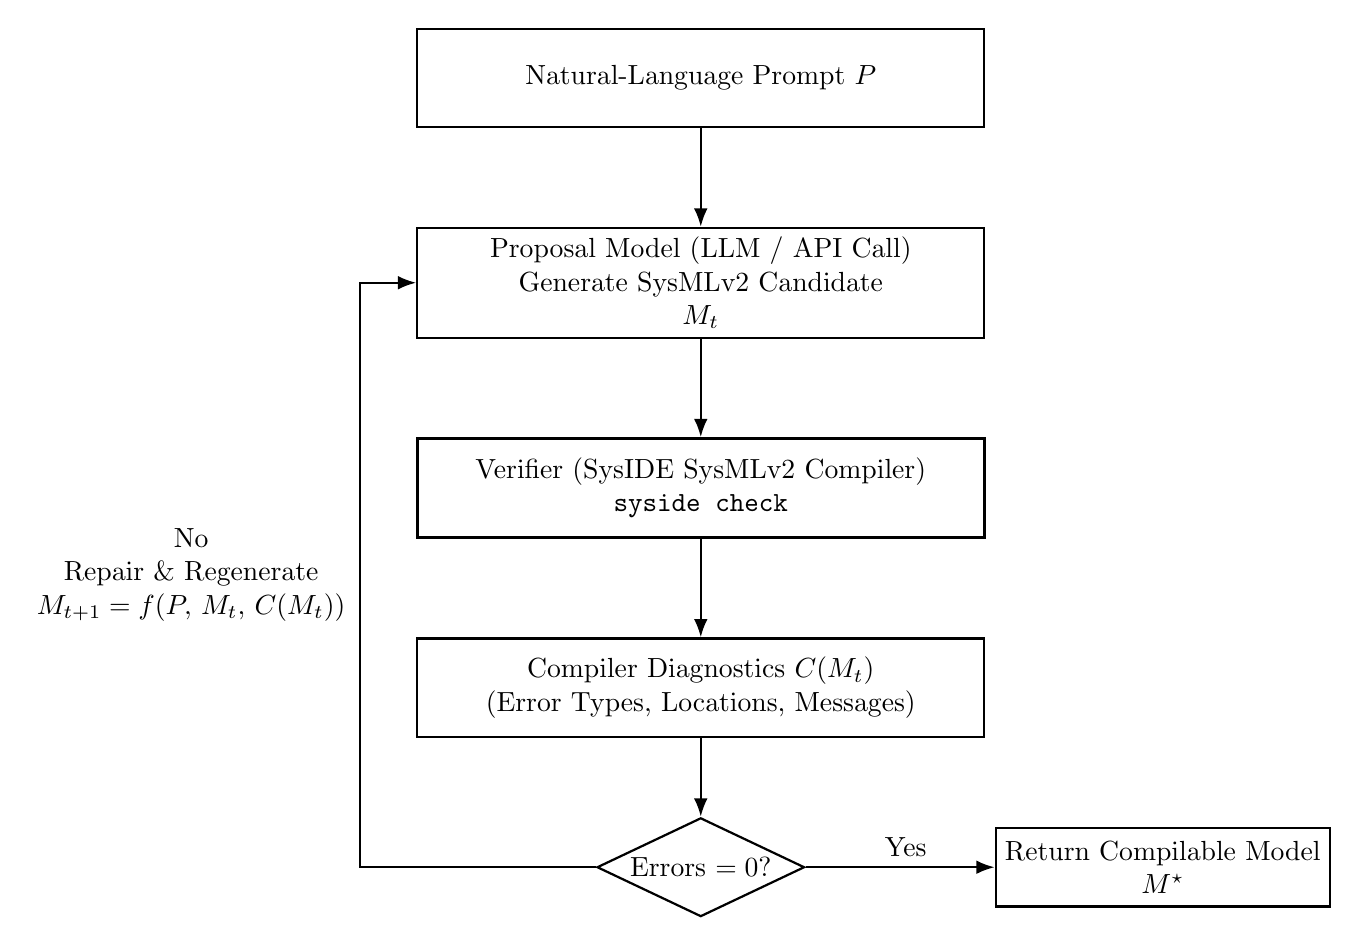
\begin{tikzpicture}[
  box/.style={draw, thick, minimum width=7.2cm, minimum height=1.25cm, align=center},
  oracle/.style={draw, very thick, minimum width=7.2cm, minimum height=1.25cm, align=center},
  decision/.style={draw, thick, diamond, aspect=2.1, inner sep=1.5pt, align=center},
  arr/.style={-Latex, thick},
  looparr/.style={-Latex, thick},
  node distance=1.25cm
]

% Nodes
\node[box] (nl) {Natural-Language Prompt $P$};

\node[box, below=of nl] (llm) {Proposal Model (LLM / API Call)\\Generate SysMLv2 Candidate\\$M_t$};

\node[oracle, below=of llm] (comp) {Verifier (SysIDE SysMLv2 Compiler)\\\texttt{syside check}};

\node[box, below=of comp] (diag) {Compiler Diagnostics $C(M_t)$\\(Error Types, Locations, Messages)};

\node[decision, below=1.0cm of diag] (dec) {Errors $=0$?};

% Forward arrows
\draw[arr] (nl) -- (llm);
\draw[arr] (llm) -- (comp);
\draw[arr] (comp) -- (diag);
\draw[arr] (diag) -- (dec);

% Return branch
\node[box, right=2.4cm of dec, minimum width=3.4cm, minimum height=1.0cm] (done)
  {Return Compilable Model\\$M^\star$};
\draw[arr] (dec) -- node[above, xshift=2pt]{Yes} (done);

% Loop arrow (No branch)
\draw[looparr]
  (dec.west) -- ++(-3,0)
  |- (llm.west);

% Loop label centered in the left loop space
\node[align=center]
  at ($(llm.west)!0.5!(dec.west)+(-4,0)$)
  {No\\Repair \& Regenerate\\$M_{t+1}=f(P,\,M_t,\,C(M_t))$};

\end{tikzpicture}
\end{document}
